\section{Умения}
%\begin{multicols}{3}             %  I am attempting to insert a second column of text next to the image,
%\begin{wraptable}[24]{l}{5.5cm}  %  but none of the wo approaches seems to work!
%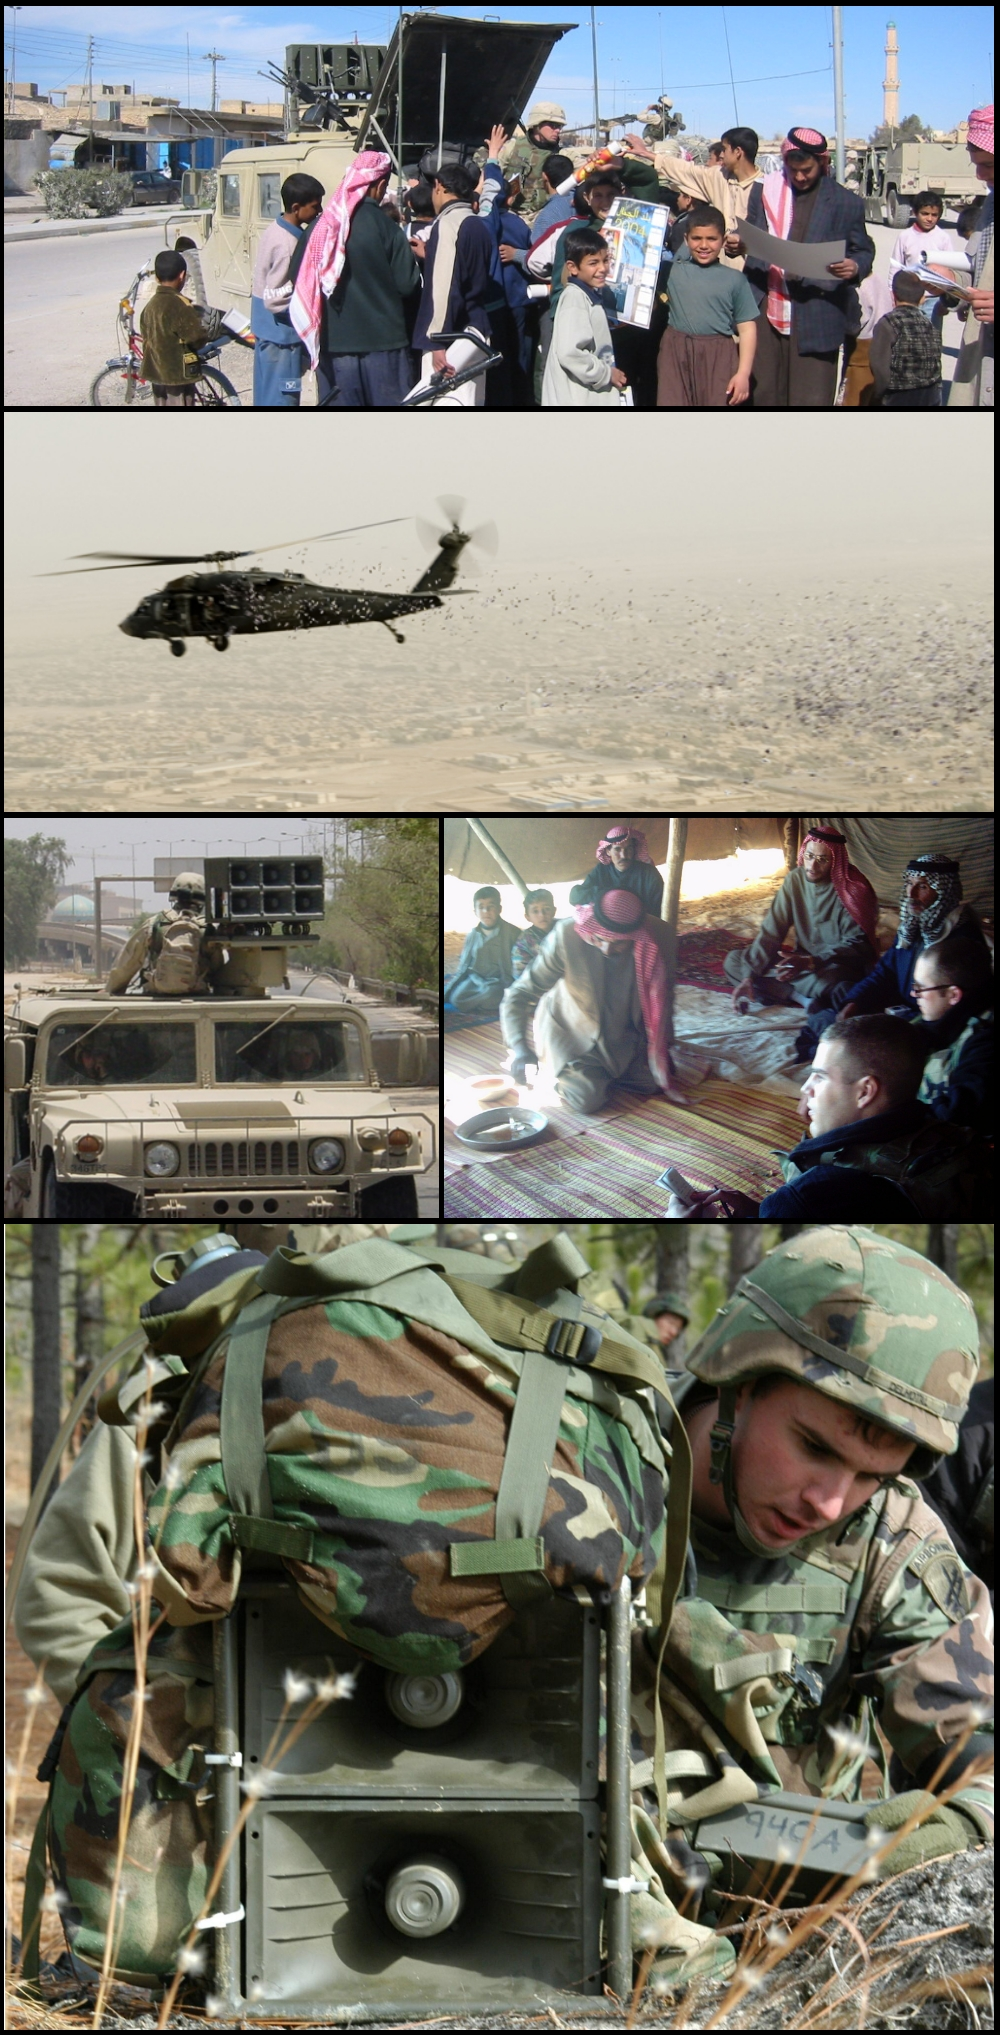
\includegraphics[width=0.3\textwidth]{../images/PSYOP.JPG}~  % TODO: include the picture when the above problem has been solved.
%\end{wraptable}
Означените със звездичка умения са събирателни понятия.
Например може да се избере \textit{елфически} език или оръжие \textit{брадва} или наука \textit{алхимия}.
\subsection{Общуване}
Лъжене (Чар)                      \\
Сплашване (Чар)                   \\
Изтезаване/Разпитване (Чар)       \\
Емпатия (Чар)                     \\
Четене по устните (Чар)           \\
Молене (Чар)                      \\

\subsection{Академични}
Език* (Ум)                        \\
Наука* (Ум)                       \\
Тактика (Ум)                      \\

\subsection{Схватки}
Оръжие* (Ловкост)                 \\
Военна машина* (Ум)               \\

\subsection{Придвижване}
Плуване (Сила)                    \\
Кaтерене (Сила)                   \\

\subsection{Занаяти}
Билкарсто (Ум)                    \\

\subsection{Епични провали}
Ако при мятане на д6* се падне -5 или +6, се мята отново.
Ако случайно се падне същото число, то се взема предивд и се продължава с мятането.
Ако крайният резултат е <0, имаме епичен провал, честито!  \\

При атака с оръжие           \\
- да го изтърве              \\
- да се сепъне               \\
- да се наръга               \\
- да се счупи                \\
- да удари някого другиго    \\
- ми нищо не се случва       \\
%\end{multicols}
